\documentclass[letterpaper,10pt,serif,draftclsnofoot,onecolumn,compsoc,titlepage]{IEEEtran}

\usepackage{graphicx}                                        
\usepackage{amssymb}                                         
\usepackage{amsmath}                                         
\usepackage{amsthm}                                          
\usepackage{cite}
\usepackage{alltt}                                           
\usepackage{float}
\usepackage{color}
\usepackage[hyphens]{url}
\usepackage{pgfgantt}
\usepackage{rotating}
\usepackage{enumitem}
\usepackage{gensymb}
\usepackage[T1]{fontenc}

\usepackage{balance}
\usepackage[TABBOTCAP, tight]{subfigure}
\usepackage{enumitem}

\usepackage{geometry}
\geometry{margin=.75in}
\usepackage{hyperref}
\usepackage{breakurl}
%\usetikzlibrary{shapes, positioning, calc}
\usepackage{caption}
\usepackage{listings}
%\usepackage[utf8]{inputenc}
%pull in the necessary preamble matter for pygments output

\usepackage{listings}
\definecolor{dkgreen}{rgb}{0,0.6,0}
\definecolor{gray}{rgb}{0.5,0.5,0.5}
\definecolor{mauve}{rgb}{0.58,0,0.82}

\lstset{frame=tb,
  %language=Java,
  aboveskip=3mm,
  belowskip=3mm,
  showstringspaces=false,
  columns=flexible,
  basicstyle={\small\ttfamily},
  numbers=none,
  %numberstyle=\tiny\color{gray},
  %keywordstyle=\color{blue},
  %commentstyle=\color{dkgreen},
  %stringstyle=\color{mauve},
  breaklines=true,
  breakatwhitespace=true,
  tabsize=3
}

%% The following metadata will show up in the PDF properties
\hypersetup{
   colorlinks = true,
   citecolor = black,
   linkcolor = black,
   urlcolor = black,
   breaklinks = true,
   pdfauthor = {Shu-Ping Chien, Brock Smedley, W Keith Striby Jr},
   pdfkeywords = {CS463 "Senior Project" Progress Report},
   pdftitle = {CS463 Spring Midterm Progress Report},
   pdfsubject = {CS463 Spring Midterm Progress Report},
   pdfpagemode = UseNone
}

\parindent = 0.0 in
\parskip = 0.1 in
\title{Winter Midterm Progress Report: Multi-Camera, SoM Based, Real-Time Video Processing for UAS and VR/AR Applications}
\author{Area 51: Shu-Ping Chien, Brock Smedley, W Keith Striby Jr \\ 06 May 2018 \\ CS463, Senior Software Engineering Project, Spring 2018}


\begin{document}
\begin{titlepage}
\maketitle

\begin{abstract}

This document highlights the group's progress made during the first half of the 
Spring 2018 term. The project is introduced along with an explanation of the 
hardware and software surrounding our product's planned solution. \\

EDIT THIS:\\
Then each group member
explains their contributions to the project, what they have remaining to complete
the projects requirements, and problems experienced with solutions if applicable. \\


\thispagestyle{empty}
\end{abstract}
\end{titlepage}

\newpage
\tableofcontents

\newpage

\section{Introduction}

\subsection{Purpose}
Our project is required to provide a video output at near real-time from a 
multi-camera input utilizing an NVIDIA Jetson TX1 or TX2 system-on-module (SoM). 
The software produced will perform image processing and edge computing on the 
camera input to display a visually enhanced and stitched video output. 
Size, weight, power, and cost (SWaP-C) requirements for the project are due 
to its application being for UAS and VR/AR, and from our system utilizing a 
mass-produced SoM, particularly the Jetson TX1 or TX2. \\

\subsection{Scope}

Application specific hardware and software are vital for the project due the the 
system requirements and constraints of the project.
The NVIDIA Jetson TX2 runs on an Ubuntu based Linux for Tegra (L4T) operating 
system created specifically for producing customized imaging, installed on a 
GPU-accelerated dual-core CPU with dual Image Signal Processors (ISPs). \\

L4T, being an Ubuntu variant, provides a friendly development interface with 
access to a large repository of additional software.NVIDIA provides the Jetson 
Software Development Pack (JetPack) 3.1 which has L4T 28.1 
and is capable of supporting a multitude of multimedia and image processing 
application program interfaces (APIs). Jetpack 
is installed on an Ubuntu host computer and is then flashed to the TX2's memory, and 
selected libraries are then installed when the TX2 is self-sustaining. \\

The cameras will utilize the most widely used camera interface for mobile applications, 
MIPI CSI-2, which is capable of supporting 1080p, 4k, and 8k video. 
A carrier board will connect the cameras to the Jetson TX2 that also provides 
additional application-specific interfaces and peripherals. \\

The software materials for this project will support the NVIDIA Jetson TX2 and 
be able to produce stitched images from cameras in near real-time. The media inputs 
from cameras are sent through  the CSI and carrier board, and then arrive at our 
software in the TX2 in raw-pixel form. The pixels are then processed through our 
GStreamer pipelines for distributing and transforming their data to the image 
processor. OpenCV libraries in our software is used to access the data in the image 
processor to produce our desired image output. The process avoids writing and 
therefore reading our input data to storage to reduce latency. The image processing 
software will utilize the images from media stream and produce streaming video 
to the display device.  \\

\subsection{Overview}

This document provides a recap of the progress made on our project through the first half
of the Spring 2018 term. The group so far has been focused on \\

EDIT:
getting the TX2 module to produce a multi-camera output with a CSI (Camera Serial Interface) module attached to the TX2 module, which allows us to connect multiple cameras to the device.
Shu-Ping Chien and W Keith Striby Jr have primarily been working in tandem so their 
contributions will be similar. Brock has spent most of the term doing research about the software we use so that it may later be scripted in order to save development time. The following 
sections reflect this progress with each group member explaining where their involvement 
with the project currently is, work remaining, problems experienced 
with solutions if applicable, and images of the hardware setups. \\ 


\section{Current Project Status}

intro?\\

\subsection{Image Processing}

types\\

\subsection{Testing}

stuff\\

\subsection{Troubleshooting Latency}

words\\

\section{Work Remaining for Project}
%Describe what you have left to do \\

\subsection{Troubleshooting Latency}

continue troubleshooting\\

\subsection{Finish Re-build of Extra TX2}

content \\

\subsection{Scripts to Build Extra TX2}

more stuff \\

\subsection{Finish Latency and Frame Rate Tests}

testing 1-2 \\

\section{Problems Experienced and Solutions (if applicable)}
%Describe any problems that have impeded your progress, with any solutions \\

intro?\\

\subsection{Latency in our GStreamer Pipelines}

it's slow \\

\subsection{Stitcher Program Lag}

it's wicked slow \\

\subsection{Latency in our Tiled Program}

it's expected due to GStreamer latency \\

\subsection{Scripts to Build Extra TX2}

issues \\

\section{Code Involved in the Project}
%Include particularly interesting pieces of code \\

insert code here \\


\section{Images of our Hardware}
%Include images of your project - screen shots, photos, etc \\

\begin{figure}[H]
	\centering
	\label{fig:TX2 module on the development kit.}
	\includegraphics[width=10cm]{images/devkit.eps}
	\caption{TX2 module on the development kit. \label{overflow}}
\end{figure}


\begin{figure}[H]
	\centering
	\label{fig:TX2 module on the development kit with the Auvidea J20 module.}
	\includegraphics[width=10cm]{images/devkit_J20.eps}
	\caption{TX2 module on the development kit with the Auvidea J20 module. \label{overflow}}
\end{figure}


\begin{figure}[H]
	\centering
	\label{fig:TX2 module connected to the Auvidea J106 carrier board and M110 motherboard, utilizing the development kit's WiFi antennas.}
	\includegraphics[width=10cm]{images/J106-M110_1.eps}
	\caption{TX2 module connected to the Auvidea J106 carrier board and M110 motherboard, utilizing the development kit's WiFi antennas. \label{overflow}}
\end{figure}


\begin{figure}[H]
	\centering
	\label{fig:A closer look at the TX2 module connected to the Auvidea J106 carrier board and M110 motherboard.}
	\includegraphics[width=10cm]{images/J106-M110_2.eps}
	\caption{A closer look at the TX2 module connected to the Auvidea J106 carrier board and M110 motherboard. \label{overflow}}
\end{figure}

\begin{figure}[H]
	\centering
	\label{fig:TX2 mounted on the Spacely Carrier Board with two CSI cameras attached.}
	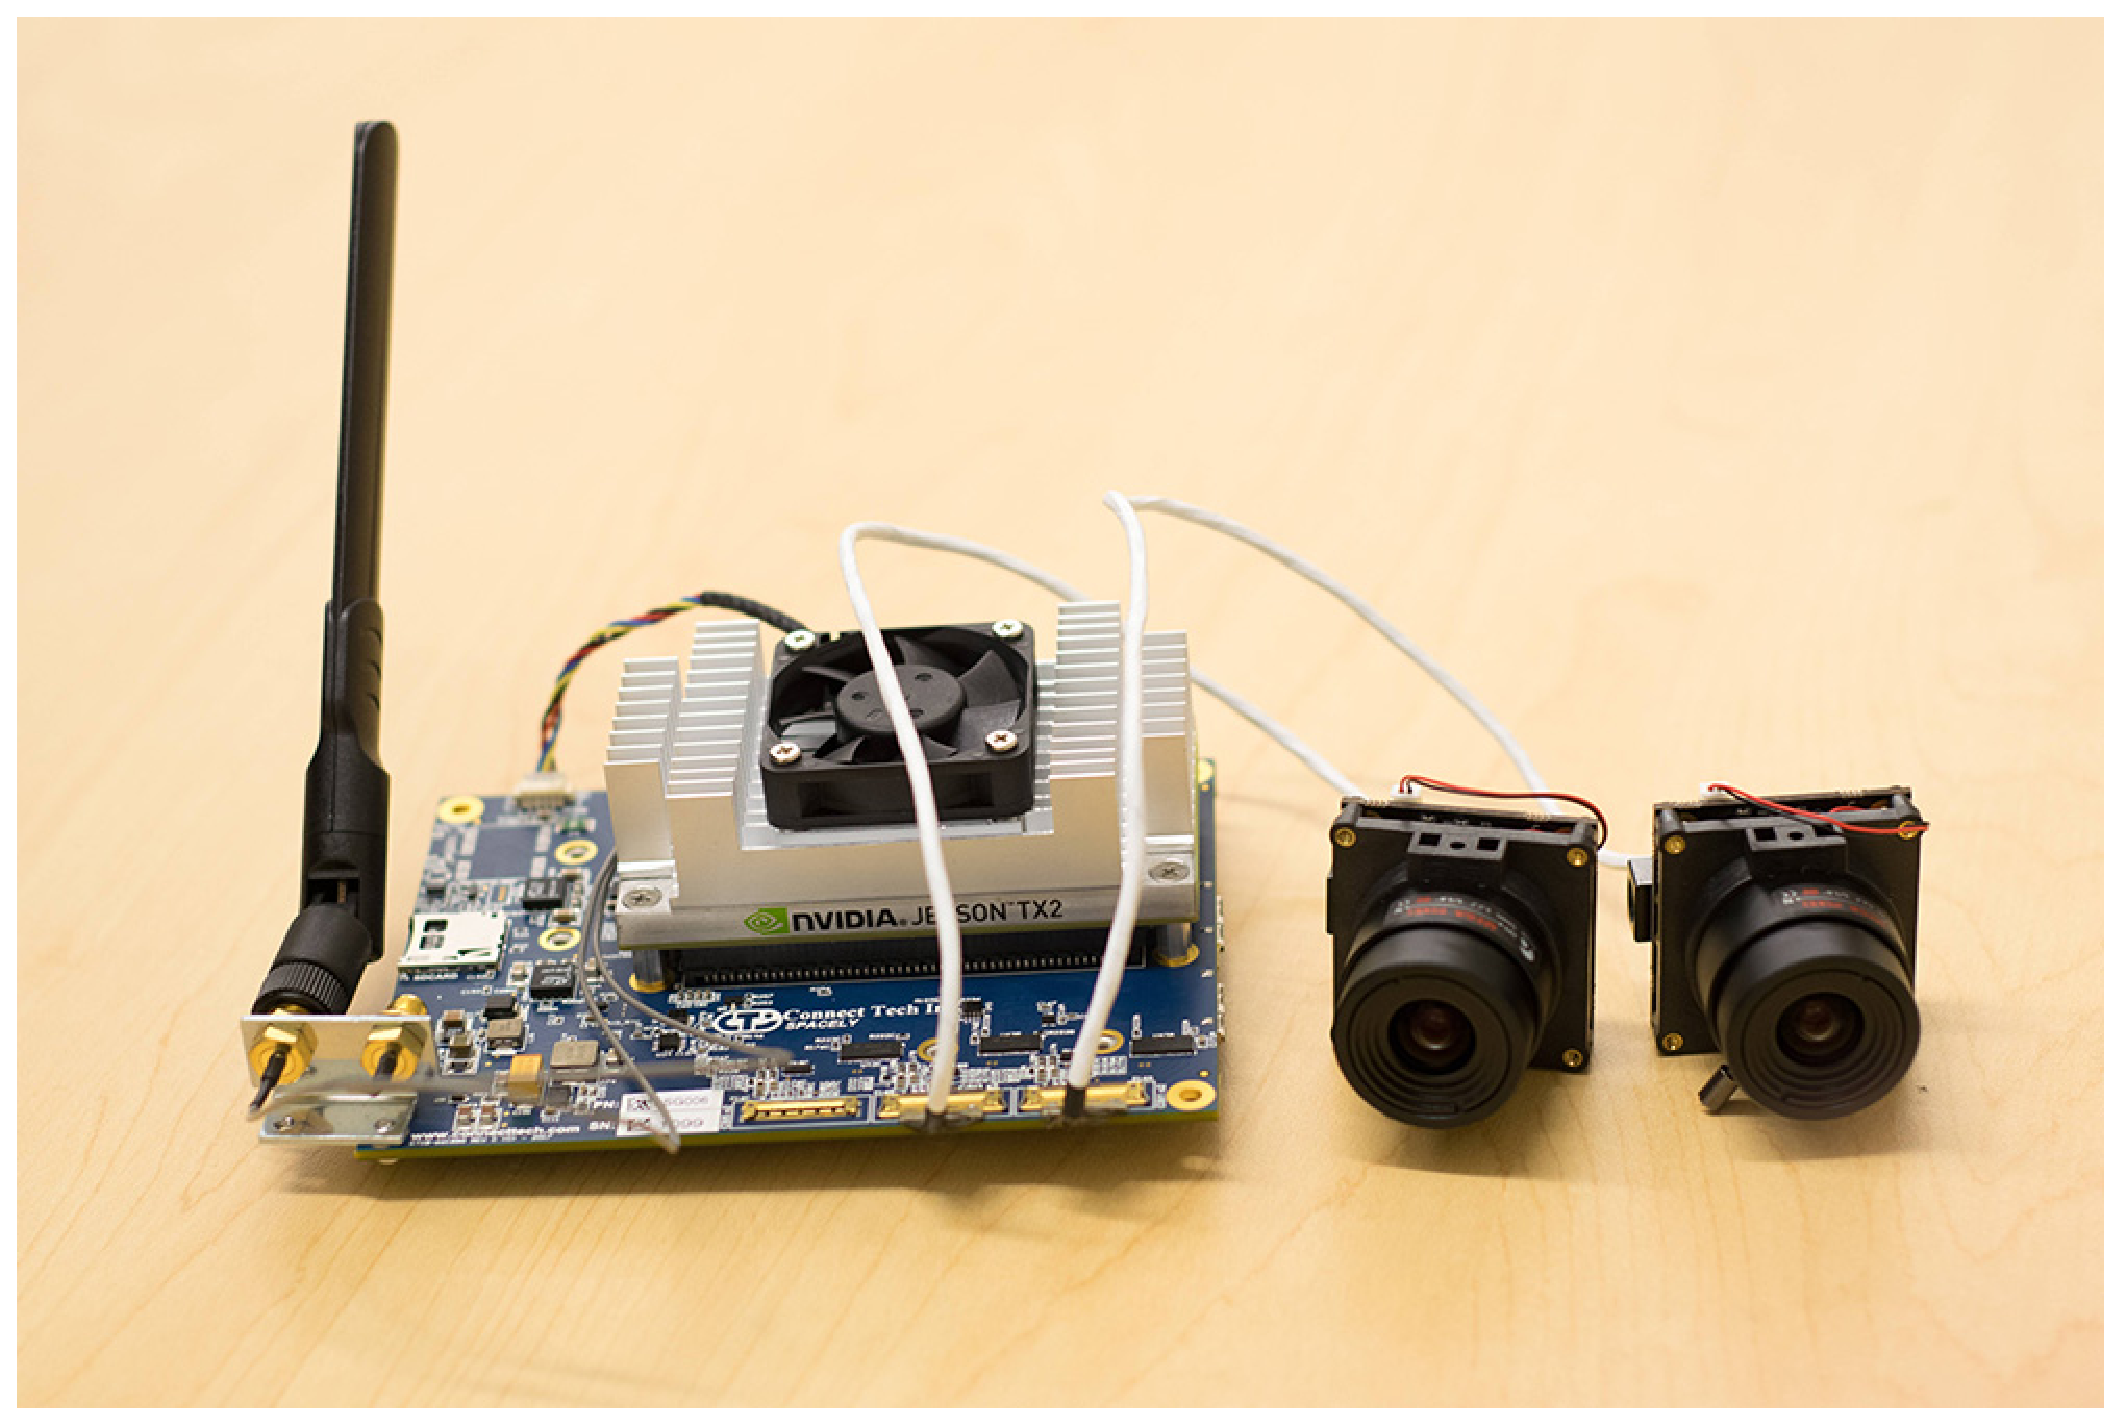
\includegraphics[width=10cm]{images/spacely.eps}
	\caption{TX2 mounted on the Spacely Carrier Board with two Leopard CSI cameras attached. \label{overflow}}
\end{figure}

%\nocite{*}
%\newpage
%\bibliographystyle{ieeetr}
%\bibliography{SpMPR_Group51}
\end{document}
